\section{Tools und Arbeitsabläufe}

Innerhalb des Cloud-Team wird jedes IT-Projekt agil nach der Scrum-Methode entwickelt.
Scrum ist ein Framework für die Entwicklung komplexer Softwareprodukte.
Sie wird von ihren Schöpfern als "ganzheitlicher, iterativer Rahmen definiert, der sich auf gemeinsame Ziele konzentriert, indem er produktiv und kreativ Produkte von höchstmöglichem Wert liefert" \cite{ScrumGuide}.
13
Es basiert auf der Unterteilung eines Projekts in "Zeit Boxen", sogenannte Sprints, die von ein paar Stunden bis zu einem Monat dauern können (in unserem Team dauert es eine Woche)

\subsection{Scrum} \label{sec:scrum}

Das Cloud-Team wendet mehrere Scrum-Methoden zur Verbesserung der
Software-Entwicklung an:

\subsubsection{Sprint Meeting}
Zu Beginn jedes Sprints trifft sich das Cloud-Team, um die verschiedenen Aufgaben für den nächsten Sprint zu planen und diese in Tickets zu organisieren.
Sie finden jeden Montag um 10 Uhr morgens statt und dauern durchschnittlich 30 Minuten.

\subsubsection{Retro Meeting}
Diese Treffen finden einmal pro Woche statt und ermöglichen jedem Teamentwickler, die guten und schlechten Punkte der vergangenen Woche zum Ausdruck zu bringen.
Dies gibt Rückmeldung über die Stimmung im Team. Sie finden jeden Donnerstag um 13.00 Uhr statt und dauern durchschnittlich 45 Minuten.

\subsubsection{Kanban board}
Die Verfolgung unserer Sprint-Tickets erfolgt über eine Kanban-Tafel.
Es handelt sich dabei um ein agiles Projektmanagement-Tool, das dazu dient, die Arbeit zu visualisieren, die laufende Arbeit zu begrenzen und die Effizienz zu maximieren.
Unsere Tabelle besteht aus 6 Spalten:

\begin{itemize}
  \item \textbf{Backlog}: Tickets geplant, aber nicht bearbeitet
  \item \textbf{Open}: Tickets, die im aktuellen Sprint erledigt werden müssen
  \item \textbf{On Hold}: Geplantes, aber für unbestimmte Zeit blockiertes Ticket
  \item \textbf{In Progress}: Die Tickets, die realisiert werden
  \item \textbf{Review}: Tickets, die derzeit einer Code Review unterzogen werden
  \item \textbf{Closed}: Tickets, die validiert und im Entwicklungszweig zusammengeführt wurden
\end{itemize}

Jedes Ticket muss begleitet sein von:
\begin{itemize}
  \item \textbf{Ein Story point}: es handelt sich um eine Zahl zwischen 1 und 8, die der geschätzten Anzahl der Stunden entspricht, die für die Erstellung des Tickets benötigt werden
  \item \textbf{eine Priorität}: dem Ticket muss Vorrang eingeräumt werden (low, medium oder high)
\end{itemize}



\subsection{Tools}

Wir verwalten all diese Prozesse sowie die Verwaltung des Codes mit verschiedenen Tools:

\subsubsection{Git}

Git\footnote{\href{https://git-scm.com/}{https://git-scm.com/}} ist ein freies und quelloffenes verteiltes Versionskontrollsystem.
Es handelt sich um ein einfaches und leistungsfähiges Tool, dessen Hauptaufgabe darin besteht, die Entwicklung der Inhalte einer Baumstruktur zu verwalten.

Git ist das Tool, aber um ein kollaboratives Projekt richtig zu verwalten, braucht das Team einen Arbeitsablauf.
Das Team hat sich für Gitflow\footnote{\href{https://www.atlassian.com/git/tutorials/comparing-workflows/gitflow-workflow}{https://www.atlassian.com/git/tutorials/comparing-workflows/gitflow-workflow}} entschieden. Dieses Workflow definiert ein striktes branch-modell, das um eine Projektfreigabe herum entworfen wurde
\footnote{Stackoverflows git-flow tag Beschreibung: \href{https://stackoverflow.com/questions/tagged/git-flow}{https://stackoverflow.com/questions/tagged/git-flow}}.

Das innerhalb des Unternehmens verwendete Modell ist recht einfach. Es besteht aus einem "main"-Branch, der die für die Code-Produktion fertige Version mit den verschiedenen Versionen enthält, den "develop"-Branch, der dem Zweig entspricht, der sich auf alle "feature"-Branch bezieht:

\begin{figure}[h]
  \centering
  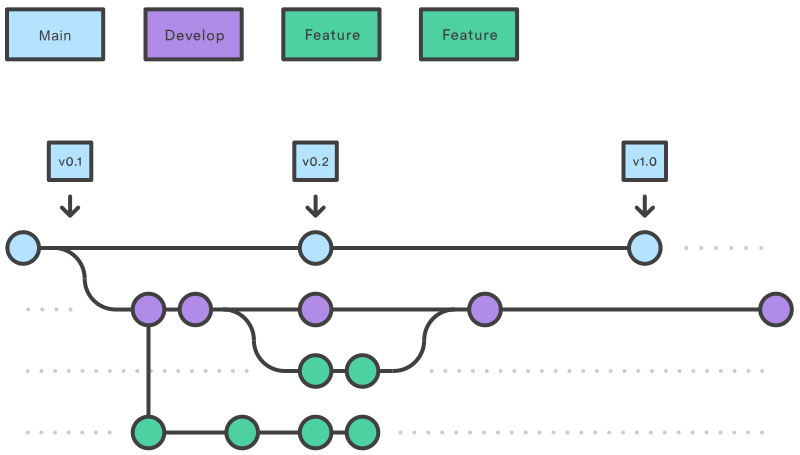
\includegraphics[width=\textwidth]{gitflow}
  \caption{Schematische Darstellung eines Git-Baums, der dem Standard von gitflow entspricht}
\end{figure}

Das Cloud-Team nahm eine Änderung am Schema vor und entfernte den branch develop, der angesichts der geringen Größe des Teams nicht relevant war.

\subsubsection{Slack}
Die Kommunikation innerhalb der Firma erfolgt mithilfe der Slack application\footnote{\href{https://slack.com/}{https://slack.com/}}.
Damit können wir einander leicht anrufen und unsere Sofortnachrichten auf verschiedene Kanälen organisieren.

\subsubsection{ClickUp} \label{sec:clickup}

ClickUp\footnote{\href{https://clickup.com/}{https://clickup.com/}} ermöglicht es uns, unseren agilen Prozess zu virtualisieren:
Tickets, Kanban-Tafel, Sprint-Planung, Roadmap, ...

\subsubsection{Google Workspace}

Die Dryad-Teams verwenden Google Workspace-Tools, um die externe Kommunikation über Google Mail, die Finanzen über Google Sheets, die Speicherung verschiedener Dateien und Bilder mit Google Drive und die Bearbeitung von Textdateien mit Google Doc zu verwalten.

\subsubsection{GitHub}

Die Verwendung von GitHub ermöglicht es, die Git-Projekte des Unternehmens online zu hosten.
Es ermöglicht uns die einfache Verwaltung unseres Quellcodes in Zusammenarbeit mit verschiedenen Features wie Code-Reviews, Veröffentlichung von npm-Paketen und kontinuierlicher Integration.

\subsection{Developer Experience}
Da der Tech Stack definiert ist, ist es möglich, das Projekt zu starten und etwas aufzubauen.
Es kann jedoch Bedenken geben, wenn mehrere Entwickler gleichzeitig am gleichen Quellcode arbeiten (Konflikte, Code-Formatierung, Sicherstellung der Gültigkeit des Codes, ...).
Deshalb ist es wichtig, bestimmte Regeln und Tools einzuführen, die es dem Entwickler ermöglichen, sich auf die eigentliche Aufgabe zu konzentrieren.
Für die Schaffung dieses Projekts war es wesentlich, die folgenden Tools/Prozesse zu implementieren, um sich in einer einfachen und homogenen Entwicklungsumgebung leicht weiterentwickeln zu können.

\subsubsection{Linter}
Ein Linter ist ein AnalyseTool für den statischen Code, das zur Kennzeichnung von Programmierfehlern, Bugs, stilistischen Fehlern und verdächtigen Konstrukten verwendet wird.
Es wurde beschlossen, den eslint\footnote{\href{https://github.com/eslint/eslint}{https://github.com/eslint/eslint}} Javascript-Linter wegen seiner Popularität und seiner verschiedenen, leicht konfigurierbaren Plugins zu verwenden (Angular\footnote{\href{https://github.com/angular-eslint/angular-eslint}{https://github.com/angular-eslint/angular-eslint}}, TypeScript\footnote{\href{https://github.com/typescript-eslint/typescript-eslint}{https://github.com/typescript-eslint/typescript-eslint}}, ...).

Eslint erlaubt es, den von jedem Entwickler geschriebenen Code zu homogenisieren.
So ist die Einrückung für alle gleich, ebenso wie Zeilenumbrüche, Leerzeichen, variable Notation, usw...

\begin{figure}[h]
  \centering
  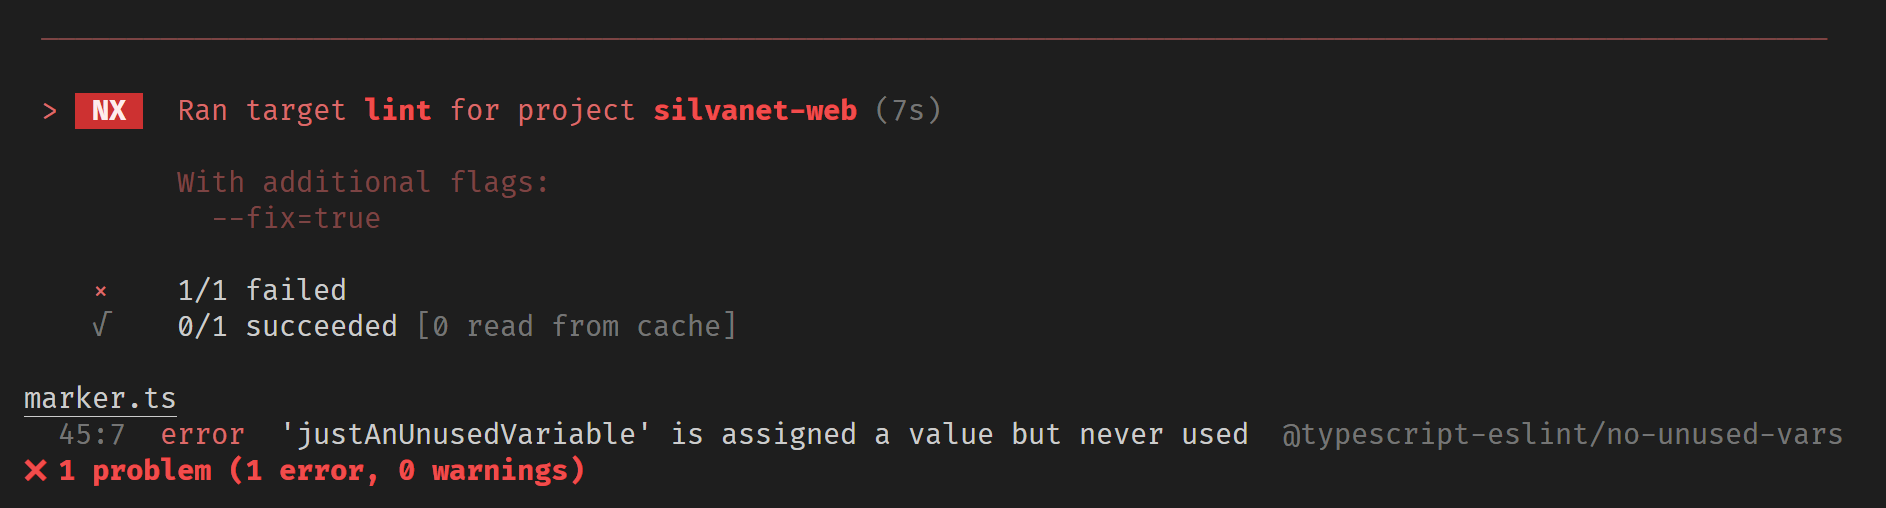
\includegraphics[width=\textwidth]{eslint_error}
  \caption{Beispiel für die Linter-Ausführung, die einen Fehler im Terminal zurückgibt}
\end{figure}

\subsubsection{TypeScript}

Typescript ist ein Tool, das entwickelt wurde, um Entwicklern die einfache Realisierung von JavaScript-Projekten zu erleichtern.
Da es aber sehr anpassungsfähig ist, muss jedoch bekannt sein, was von diesem Tool erwartet wird und wie es verwendet werden soll.

Es wurde daher beschlossen, TypeScript mit einer hohen Anforderung zu konfigurieren.
Daher muss alles typisiert werden (Variablen, Funktionen, Parameter), damit jeder Entwickler leichter verstehen kann, was an jeder Stelle im Code geschieht.
Darüber hinaus ist der "beliebige" Typ verboten, da er die Verwendung von TypeScript überflüssig macht.

Dies mag dem DX-Prinzip zuwiderlaufen, da es anfangs viele Einschränkungen mit sich bringt, aber nach einer kurzen Anpassungszeit kommen die Vorteile eines stark typisierten Codes schnell zum Tragen und verbessern die Erfahrung des Entwicklers erheblich.

\subsubsection{Drone CI}

In jedem Beruf ist es sehr ärgerlich, immer wieder die gleichen Aufgaben auszuführen.
In der Entwicklungswelt müssen wir zum Beispiel sicherstellen, dass der zur Produktion geschickte Code dem Linters-Standard entspricht, sich problemlos kompilieren lässt und vorher alle Tests besteht.
Ständig darauf achten zu müssen, sie nicht zu vergessen, belastet die Entwickler unnötig mental.

Aus diesem Grund verwendet das Unternehmen ein kontinuierliches Integrations-Tool, Drone CI\footnote{\href{https://www.drone.io/}{https://www.drone.io/}}.
Es ist sehr kompatibel mit GitHub und ermöglicht, bestimmte Aufgaben auszuführen, wenn Code auf GitHub gepusht wird.

Seine große Stärke ist die Einfachheit der Konfiguration. Es muss nämlich nach der Verknüpfung von travis mit dem GitHub-Projekt nur noch eine einfache \lstinline!.drone.yml!-Datei an der Root des Projekts erstellt und bearbeitet werden.
